\documentclass[11pt]{article}
\usepackage[utf8]{inputenc}
\usepackage[T1]{fontenc}
\usepackage{amsmath}
\usepackage{amssymb} % Needed for \eth
\usepackage{graphicx}
\usepackage{geometry}
\usepackage{tikz}
\usepackage{pgfplots} % For plots
\usepackage{ulem}     % For underline, using normalem to avoid messing with \emph

\geometry{a4paper, margin=1in}
\usetikzlibrary{positioning, arrows.meta, shapes.geometric, patterns} % For TikZ diagrams
\pgfplotsset{compat=1.18} % Use a recent PGFPlots version

% Custom commands (optional)
\newcommand{\avg}[1]{\overline{#1}}
\newcommand{\prob}[1]{P(#1)}
\newcommand{\ProbDens}[1]{\mathcal{P}(#1)} % Using script P for density
\newcommand{\vect}[1]{\vec{#1}}
\newcommand{\dd}[1]{\mathrm{d}#1} % Differential d
\newcommand{\pderiv}[2]{\frac{\partial #1}{\partial #2}}
\newcommand{\deriv}[2]{\frac{\mathrm{d} #1}{\mathrm{d} #2}}
\newcommand{\muState}{\mu\text{-state}} % Microstate
\newcommand{\OmegaE}{\Omega(E)}
\newcommand{\omegaE}{\omega(E)}
\newcommand{\PhiE}{\Phi(E)}
\newcommand{\deltaE}{\delta E}
\newcommand{\ethbar}{\text{\it{đ}}} % \eth symbol for inexact differential
\newcommand{\kb}{k_B} % Boltzmann constant
\newcommand{\gasR}{R} % Ideal gas constant

\title{Physics 415 - Lecture 14: Thermodynamic Applications}
\date{February 21, 2025}
\author{} % Author not specified

\begin{document}

\maketitle
\thispagestyle{empty}

\section*{Summary}

\begin{itemize}
    \item Fundamental Relation: $dE = T dS - p dV$.
    \item Maxwell Relations (derived from exactness of $dE, dF, dH, dG$):
    \begin{align*} \left( \pderiv{T}{V} \right)_S &= - \left( \pderiv{p}{S} \right)_V & \left( \pderiv{T}{p} \right)_S &= \left( \pderiv{V}{S} \right)_p \\ \left( \pderiv{S}{V} \right)_T &= \left( \pderiv{p}{T} \right)_V & \left( \pderiv{S}{p} \right)_T &= -\left( \pderiv{V}{T} \right)_p \end{align*}
    \item Heat Capacity: $\ethbar Q|_x = C_x dT$, and $C_x = T (\partial S / \partial T)_x$.
    \item Relation between heat capacities: $C_p - C_V = TV \alpha_p^2 / K_T$, where
    \begin{itemize}
        \item Thermal expansion coefficient: $\alpha_p = \frac{1}{V} (\partial V / \partial T)_p$
        \item Isothermal compressibility: $K_T = -\frac{1}{V} (\partial V / \partial p)_T$
    \end{itemize}
\end{itemize}

\textbf{Check for Ideal Gas:} $pV = \nu \gasR T$.
\[ \alpha_p = \frac{1}{V} \left( \pderiv{V}{T} \right)_p = \frac{1}{V} \left( \pderiv{(\nu \gasR T/p)}{T} \right)_p = \frac{1}{V} \frac{\nu \gasR}{p} = \frac{\nu \gasR}{pV} = \frac{1}{T} \]
\[ K_T = -\frac{1}{V} \left( \pderiv{V}{p} \right)_T = -\frac{1}{V} \left( \pderiv{(\nu \gasR T/p)}{p} \right)_T = -\frac{1}{V} \left( -\frac{\nu \gasR T}{p^2} \right) = \frac{\nu \gasR T}{V p^2} = \frac{pV}{V p^2} = \frac{1}{p} \]
Substitute into the general relation:
\[ C_p - C_V = TV \frac{(1/T)^2}{(1/p)} = \frac{V p}{T} = \frac{\nu \gasR T}{T} = \nu \gasR \]
In molar terms: $c_p - c_v = \gasR$. $\checkmark$

\section*{Third Law Implications for Response Functions}

The Third Law ($S \to S_0$ as $T \to 0$, where $S_0$ is constant) has interesting implications for specific heats and other response functions at low temperatures.
\begin{itemize}
    \item \textbf{Heat Capacities:} $C_V = T (\partial S / \partial T)_V$. Since $S$ approaches a constant $S_0$ as $T \to 0$, the derivative $(\partial S / \partial T)_V$ must remain finite (or go to zero) for $S$ to be well-behaved near $T=0$. Therefore, $C_V \to 0$ as $T \to 0$.
    Alternatively, $S(T) - S(0) = \int_0^T (C_V(T')/T') dT'$. For this integral to converge at the lower limit $T'=0$, we must have $C_V(T') \to 0$ as $T' \to 0$.
    Similarly, it follows that $C_p = T (\partial S / \partial T)_p \to 0$ as $T \to 0$.

    \item \textbf{Thermal Expansivity:} $\alpha_p = \frac{1}{V} (\partial V / \partial T)_p$. Using Maxwell Relation (4), $(\partial V / \partial T)_p = -(\partial S / \partial p)_T$. As $T \to 0$, $S \to S_0$, where $S_0$ is independent of external parameters like $p$. Thus, $(\partial S / \partial p)_T \to (\partial S_0 / \partial p)_T = 0$.
    Therefore, $\alpha_p \to 0$ as $T \to 0$.

    \item \textbf{Isothermal Compressibility:} $K_T = -\frac{1}{V} (\partial V / \partial p)_T$. This involves purely mechanical quantities and does not necessarily go to zero as $T \to 0$. It typically approaches a finite positive value.

    \item \textbf{Relation $C_p - C_V$:}
    $C_p - C_V = TV \alpha_p^2 / K_T$.
    Assume typical low-temperature behavior based on QM models (e.g., for solids/fermions) $S \sim T^n$ for some $n>0$.
    Then $C_V = T(\partial S/\partial T)_V \sim T^n$.
    Also, $(\partial S/\partial p)_T$. If $S(T,p) \approx S_0(p) + A(p) T^n$, then $(\partial S/\partial p)_T = S_0'(p) + A'(p)T^n$. For $S\to S_0$ (const), maybe $S_0'(p)=0$ and $A'(p)$ finite? Let's assume $(\partial S/\partial p)_T \sim T^n$ as suggested by the source notes based on power counting.
    Then $\alpha_p = -(1/V)(\partial S/\partial p)_T \sim T^n$.
    $C_p - C_V \sim T V (T^n)^2 / K_T \sim T^{2n+1}$ (assuming $V, K_T$ finite at $T=0$).
    The ratio $\frac{C_p - C_V}{C_V} \sim \frac{T^{2n+1}}{T^n} = T^{n+1}$. Since $n>0$, this ratio $\to 0$ as $T \to 0$.
    The difference $C_p - C_V$ goes to zero faster than the specific heats themselves.
\end{itemize}
Note: Specific heats of the classical ideal gas ($C_V = \frac{3}{2}\nu R$, $C_p = \frac{5}{2}\nu R$) are constant and fail to satisfy $C_V \to 0, C_p \to 0$ as $T \to 0$. This is because classical theory breaks down at low T, where QM effects become important.

\section*{Reconstruction of Entropy and Energy}

Take $(T,V)$ as independent variables describing the macroscopic system.
Question: What information do we need to reconstruct $S(T,V)$ and $E(T,V)$?

\textbf{Entropy $S(T,V)$:}
\[ dS = \left( \pderiv{S}{T} \right)_V dT + \left( \pderiv{S}{V} \right)_T dV \]
Using $C_V = T (\partial S / \partial T)_V$ and Maxwell relation $(\partial S / \partial V)_T = (\partial p / \partial T)_V$:
\[ dS = \frac{C_V(T,V)}{T} dT + \left( \pderiv{p}{T} \right)_V dV \]
To integrate this to find $S(T,V)$ relative to a reference state $(T_0, V_0)$, we need to know $C_V(T,V)$ and the equation of state $p=p(T,V)$ (to find the partial derivative $(\partial p / \partial T)_V$).

In fact, the dependence of $C_V$ on $V$ is determined by the equation of state:
\[ \left( \pderiv{C_V}{V} \right)_T = \pderiv{}{V} \left[ T \left( \pderiv{S}{T} \right)_V \right]_T = T \pderiv[2]{S}{V \partial T} = T \pderiv[2]{S}{T \partial V} \]
\[ = T \pderiv{}{T} \left[ \left( \pderiv{S}{V} \right)_T \right]_V \]
Using Maxwell relation $(\partial S / \partial V)_T = (\partial p / \partial T)_V$:
\[ \left( \pderiv{C_V}{V} \right)_T = T \left( \pderiv[2]{p}{T^2} \right)_V \]
So, if $C_V(T, V_0)$ is known at a single volume $V_0$ (e.g., from experiment or theory), we can find $C_V(T,V)$ at any other volume using the equation of state $p(T,V)$:
\[ C_V(T,V) = C_V(T,V_0) + \int_{V_0}^V \left( \pderiv{C_V}{V'} \right)_T dV' = C_V(T,V_0) + \int_{V_0}^V T \left( \pderiv[2]{p(T,V')}{T^2} \right)_V dV' \]
Therefore, $S(T,V)$ can be reconstructed from knowledge of the equation of state $p(T,V)$ and the heat capacity $C_V(T)$ at a single volume (or density).
Explicitly, integrating $dS$:
\[ S(T,V) - S(T_0, V_0) = \int_{(T_0,V_0)}^{(T,V)} \left[ \frac{C_V(T',V')}{T'} dT' + \left( \pderiv{p(T',V')}{T'} \right)_V dV' \right] \]
A convenient integration path is $(T_0, V_0) \to (T_0, V) \to (T, V)$:
\[ S(T,V) - S(T_0, V_0) = \int_{V_0}^V \left( \pderiv{p(T_0,V')}{T} \right)_V dV' + \int_{T_0}^T \frac{C_V(T',V)}{T'} dT' \]

\textbf{Internal Energy $E(T,V)$:}
From $dE = T dS - p dV$, substitute $dS = (C_V/T) dT + (\partial p/\partial T)_V dV$:
\[ dE = T \left[ \frac{C_V}{T} dT + \left( \pderiv{p}{T} \right)_V dV \right] - p dV \]
\[ dE = C_V dT + \left[ T \left( \pderiv{p}{T} \right)_V - p \right] dV \]
Comparing with $dE = (\partial E/\partial T)_V dT + (\partial E/\partial V)_T dV$:
\[ \left( \pderiv{E}{T} \right)_V = C_V(T,V) \]
\[ \left( \pderiv{E}{V} \right)_T = T \left( \pderiv{p}{T} \right)_V - p \]
(This confirms the relation $(\partial E/\partial V)_T = T^2 (\partial (p/T)/\partial T)_V$ derived earlier).
$E(T,V)$ can again be obtained by integration from a reference state $(T_0, V_0)$ using knowledge of $C_V(T)$ (at some reference volume) and the equation of state $p(T,V)$.

\section*{Free Expansion (Joule Expansion)}

This example illustrates some general methods in macro thermodynamics.
Consider a gas initially in equilibrium at temperature $T_1$ and volume $V_1$ in one side of an insulated container. The other side is evacuated. The partition is removed, and the gas expands freely into the total volume $V_2$. The system is thermally isolated throughout.

\begin{center}
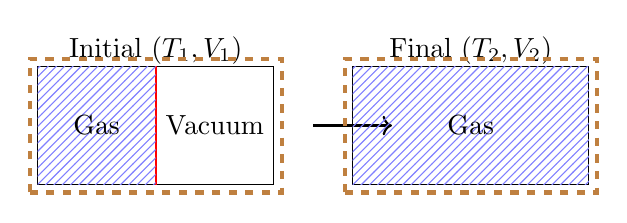
\begin{tikzpicture}
    % Initial State
    \node at (-1.5, 1.7) {Initial ($T_1, V_1$)};
    \draw (-3,0) rectangle (0,1.5); % Container
    \draw[thick, red] (-1.5, 0) -- (-1.5, 1.5); % Partition
    \fill [pattern=north east lines, pattern color=blue!50] (-3,0) rectangle (-1.5, 1.5); % Gas
    \node at (-2.25, 0.75) {Gas};
    \node at (-0.75, 0.75) {Vacuum};
    % Insulation
    \draw[line width=1.5pt, brown, dashed] (-3.1, -0.1) rectangle (0.1, 1.6);

    % Arrow
    \draw [->, thick] (0.5, 0.75) -- (1.5, 0.75);

    % Final State
    \begin{scope}[xshift=4cm]
        \node at (-1.5, 1.7) {Final ($T_2, V_2$)};
        \draw (-3,0) rectangle (0,1.5); % Container
        \fill [pattern=north east lines, pattern color=blue!50] (-3,0) rectangle (0, 1.5); % Gas expanded
        \node at (-1.5, 0.75) {Gas};
        % Insulation
        \draw[line width=1.5pt, brown, dashed] (-3.1, -0.1) rectangle (0.1, 1.6);
    \end{scope}
\end{tikzpicture}
\end{center}

Question: What is the final temperature $T_2$, after the system reaches equilibrium in volume $V_2$?
\begin{itemize}
    \item System is thermally isolated $\implies Q=0$.
    \item System does no work on surroundings (expansion into vacuum) $\implies W=0$.
    \item First Law: $\Delta E = Q - W = 0$.
    \item The internal energy of the system does not change: $E(T_1, V_1) = E(T_2, V_2)$.
\end{itemize}
This is an implicit equation for $T_2$.

\textbf{Ideal Gas Case:} For an ideal gas, $E=E(T)$ only (independent of $V$).
The condition $E(T_1) = E(T_2)$ implies $T_1 = T_2$.
For an ideal gas, there is no change in temperature in a free expansion.

\textbf{General Case:} We need to know $E(T,V)$ to determine $T_2$.
The process itself (removing partition) is highly irreversible, not quasi-static. However, the initial and final states are equilibrium states. We can relate them by the condition $E=\text{constant}$.

\begin{center}
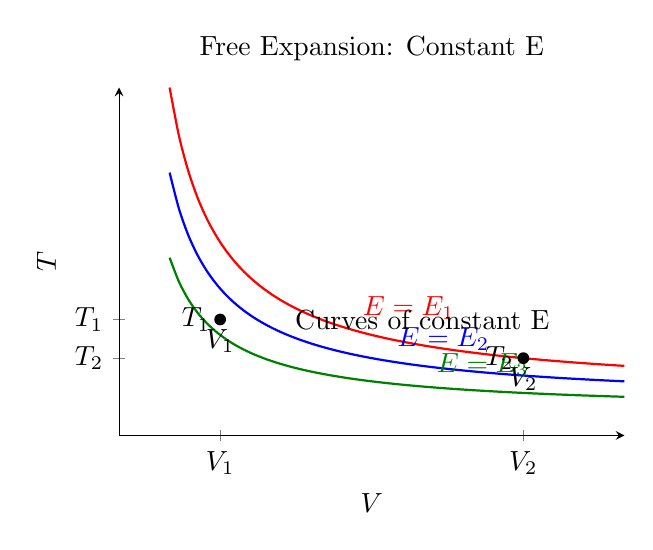
\begin{tikzpicture}
\begin{axis}[
    axis lines=left, xlabel=$V$, ylabel=$T$,
    xmin=0, ymin=0,
    width=8cm, height=6cm,
    xtick={1, 4}, xticklabels={$V_1$, $V_2$},
    ytick={2, 3}, yticklabels={$T_2$, $T_1$}, % Example if T decreases
    title={Free Expansion: Constant E}
]
\addplot [domain=0.5:5, samples=50, smooth, thick, red] {4/x + 1} node[pos=0.7, anchor=south west] {$E=E_1$}; % Example E=const curve 1
\addplot [domain=0.5:5, samples=50, smooth, thick, blue] {3/x + 0.8} node[pos=0.7, anchor=south west] {$E=E_2$}; % Example E=const curve 2
\addplot [domain=0.5:5, samples=50, smooth, thick, green!50!black] {2/x + 0.6} node[pos=0.7, anchor=south west] {$E=E_3$}; % Example E=const curve 3

% Points
\coordinate (P1) at (axis cs:1, 3); % E=E1, T=T1, V=V1
\coordinate (P2) at (axis cs:4, 1.75); % E=E1, T=T2, V=V2 (Example for E1 curve: 4/4+1 = 2, not 1.75... using a point on the curve)
\coordinate (P2_actual) at (axis cs:4, {4/4+1}); % T=2
\node at (P1) [circle, fill=black, inner sep=1.5pt] {};
\node at (P2_actual) [circle, fill=black, inner sep=1.5pt] {};
\draw [dashed] (P1 |- 0,3) node[left]{$T_1$} -- (P1) -- (1,0 |- P1) node[below]{$V_1$};
\draw [dashed] (P2_actual |- 0,2) node[left]{$T_2$} -- (P2_actual) -- (4,0 |- P2_actual) node[below]{$V_2$};
\node at (axis cs: 3, 3) {Curves of constant E};
\end{axis}
\end{tikzpicture}
\end{center}
The initial state $(T_1, V_1)$ and final state $(T_2, V_2)$ lie on the same curve of constant $E$.

To see how $T$ changes with $V$ at constant $E$, consider the derivative $(\partial T / \partial V)_E$ (Joule coefficient $\mu_J$).
From $dE = (\partial E/\partial T)_V dT + (\partial E/\partial V)_T dV$, if $dE=0$:
\[ \left( \pderiv{T}{V} \right)_E = - \frac{(\partial E / \partial V)_T}{(\partial E / \partial T)_V} = -\frac{1}{C_V} \left( \pderiv{E}{V} \right)_T \]
We previously showed (from $dS$ exactness) that $(\partial E / \partial V)_T = T (\partial p / \partial T)_V - p$.
\[ \left( \pderiv{T}{V} \right)_E = -\frac{1}{C_V} \left[ T \left( \pderiv{p}{T} \right)_V - p \right] = \frac{1}{C_V} \left[ p - T \left( \pderiv{p}{T} \right)_V \right] \]
Using Maxwell relation $(\partial p/\partial T)_V = (\partial S/\partial V)_T$:
\[ \left( \pderiv{T}{V} \right)_E = \frac{1}{C_V} \left[ p - T \left( \pderiv{S}{V} \right)_T \right] \]
We also showed $(\partial p / \partial T)_V = \alpha_p / K_T$.
\[ \implies \left( \pderiv{T}{V} \right)_E = \frac{1}{C_V} \left( p - \frac{T \alpha_p}{K_T} \right) \]
For ideal gas, $\alpha_p=1/T, K_T=1/p$, so $p - T\alpha_p/K_T = p - T(1/T)/(1/p) = p - p = 0$. So $(\partial T/\partial V)_E=0$.
For a finite change, we integrate along a (fictitious) quasi-static path of constant E:
\[ T_2 - T_1 = \int_{V_1}^{V_2} \left( \pderiv{T}{V} \right)_E dV \]
In principle, free expansion could be used to cool (or heat) non-ideal gases, but the effect $(\partial T/\partial V)_E$ is usually very small.

\textbf{Entropy Change in Free Expansion:}
The process is irreversible, so $\Delta S_{tot} > 0$. Since the system is isolated, $\Delta S_{tot} = \Delta S_{system}$. We expect $\Delta S > 0$.
To calculate $\Delta S = S(T_2, V_2) - S(T_1, V_1)$, we use the fact that $S$ is a state function and devise any reversible path between the initial and final states. Since $E$ is constant, the initial and final states lie on a curve $E(T,V)=E_1$. We can integrate $dS$ along this curve.
From $dE = T dS - p dV$, if $dE=0$, then $T dS = p dV \implies dS = (p/T) dV$ along a path of constant $E$.
\[ \Delta S = S(E_1, V_2) - S(E_1, V_1) = \int_{V_1}^{V_2} \left( \pderiv{S}{V} \right)_E dV' \]
We need $(\partial S/\partial V)_E$. From $dS = (1/T)dE + (p/T)dV$, we have $(\partial S/\partial V)_E = p(E,V)/T(E,V)$.
\[ \Delta S = \int_{V_1}^{V_2} \frac{p(E_1, V')}{T(E_1, V')} dV' \]

\textbf{Ideal Gas Case:} $E=E(T)$, so constant $E$ implies constant $T=T_1$. $p/T = N/V$.
\[ \Delta S = \int_{V_1}^{V_2} \frac{N}{V'} dV' = N [\ln V']_{V_1}^{V_2} = N \ln \left( \frac{V_2}{V_1} \right) \]
Since $V_2 > V_1$ (expansion), $\ln(V_2/V_1) > 0$, so $\Delta S > 0$. The entropy increases, confirming the process is irreversible.

\end{document}